\chapter{Empirical studies}
\label{empirical}

\section{Introduction}
%=============================
In this chapter the runtime of three Parallel GA(PGA) implementations (discussed in previous chapter) are compared against the sequential GA implementation. Each implementation is compared and contrasted with SGA. We focused this study on to observe the program runtime by varying number of processes and by varying the population size. These experiments were carried out on a physical Beowulf cluster setup as described in Section \ref{test_config} with test configurations shown in Section \ref{test_config}. Results may vary using other cluster configuration.


Even though we kept the free-parameter's values consistent throughout the experiments there are other constraints on which we do not have any explicit control to fine tune them. This constraints include Linux schedular (which runs other system daemons and services), and network system overhead. Extra care was taken to ensure no other programs were running during the experiments and network activities were minimum. To further validate our experiments data  statistical method of confidence interval were used. 

In statistics, a confidence interval (CI) is a type of interval estimation of a random variable (in this experiment which is the program run time). It is an observed interval (i.e. calculated from the observations). In principle this interval is different from sample to sample, that potentially includes the unobservable true parameter of interest. How frequently the observed interval contains the true parameter if the experiment is repeated is called the confidence level. If confidence intervals are constructed in separate experiments on the same population following the same process, the proportion of such intervals that contain the true value of the parameter will match the given confidence level\citep{cox1979theoretical}. Whereas two-sided confidence limits form a confidence interval, and one-sided limits are referred to as lower/upper confidence bounds (or limits).

All of the sample runtime data gathered here are averaged from 20 runs. Due to time constraint sample size is kept 20 which means we run each program for 20 times and recorded the time taken from start to finish for each run. To calculate CI the average \textbf{$ \bar{x} $ } and standard deviation \textbf{$ \delta $} is calculated of these 20 data set. Then the CI is calculated using following formula where \textbf{$z = 1.96 $} for 95\% CI:
\[
	Upper Limit = \bar{x} + z (\delta/\sqrt{20})
\]
\[
	Lower Limit = \bar{x} - z (\delta/\sqrt{20})
\]

Table \ref{tab:emp_table_1} shows the data of average running time for all three implementation of PGA using a population size 5000 with their upper and lower bound with 95\% confidence level. Which means that 95\% of time time the true value of the program runtime is within our confidence interval. After any particular sample is taken, given that exactly same configuration were used, the program runtime should be within these intervals shown in the Table \ref{tab:emp_table_1} 95\% of the time.


\begin{table}[!htb]
\centering
\caption{A sample runs using population size of 5000 to determine average runtime(seconds) for PGA v1, PGA v2 and PGA v3.}
\label{tab:emp_table_1}
\begin{tabular}{|l|l|l|l|}
\hline
RUN                & PGA v1   & PGA v2  & PGA v3  \\ \hline
0                  & 14.8262 & 5.0441 & 1.7067 \\ \hline
1                  & 14.7368 & 5.0157 & 1.9845 \\ \hline
2                  & 15.0571 & 4.9169 & 1.7116 \\ \hline
3                  & 15.0404 & 4.9911 & 1.6933 \\ \hline
4                  & 16.2858 & 4.9056 & 1.6935 \\ \hline
5                  & 14.5847 & 5.0745 & 1.7016 \\ \hline
6                  & 14.7812 & 5.0515 & 1.6980 \\ \hline
7                  & 15.4188 & 5.0403 & 1.7069 \\ \hline
8                  & 16.4531 & 4.9878 & 1.6974 \\ \hline
9                  & 16.9943 & 4.8959 & 1.7039 \\ \hline
10                 & 15.7324 & 4.9217 & 1.6986 \\ \hline
11                 & 14.4173 & 4.9180 & 1.7055 \\ \hline
12                 & 14.6054 & 5.0879 & 1.7063 \\ \hline
13                 & 14.8513 & 4.9155 & 1.7112 \\ \hline
14                 & 15.4737 & 4.9294 & 1.7024 \\ \hline
15                 & 14.4207 & 5.0595 & 1.6966 \\ \hline
16                 & 16.0418 & 5.0947 & 1.7095 \\ \hline
17                 & 16.8885 & 5.0685 & 1.6873 \\ \hline
18                 & 15.0276 & 4.9684 & 1.7136 \\ \hline
19                 & 16.4414 & 4.9665 & 1.7077 \\ \hline
\multicolumn{4}{|l|}{}                         \\ \hline
Average            & 15.4039 & 4.9927 & 1.7168 \\ \hline
Standard Deviation & 0.8162  & 0.0670 & 0.0618 \\ \hline
CI (95\%)          & 0.3577  & 0.0294 & 0.0271 \\ \hline
\multicolumn{4}{|l|}{}                         \\ \hline
Upper Limit        & 15.7616 & 5.0220 & 1.7439 \\ \hline
Lower Limit        & 15.0462 & 4.9633 & 1.6897 \\ \hline
\end{tabular}
\end{table}


Using this method all data for the experiments listed below were validated. The results shown for these experiments are the average of 20 runs.

\section{Experiments using PGA v1}
%=============================

\subsection{Experiment 1: Varying number of processes}

\subsubsection{Objective}
Comparison of PGA v1 runtime vs. SGA runtime by varying the number of processes the work is distributed for the PGA program to see the speedup gain using a fixed population size 5000.

\begin{table}[H]
\centering
\caption{Experiment 1 data using PGA v1}
\label{tab:pga1_node}
\begin{tabular}{|l|l|l|l|}
\hline
\# Process(es) & SGA     & PGA     & speedup \\ \hline
1        & 12.8789 & 12.8887 & 0.9992  \\ \hline
2        & 12.8789 & 12.8464 & 1.0025  \\ \hline
3        & 12.8789 & 13.1183 & 0.9818  \\ \hline
4        & 12.8789 & 13.1585 & 0.9788  \\ \hline
5        & 12.8789 & 13.4671 & 0.9563  \\ \hline
6        & 12.8789 & 15.3387 & 0.8396  \\ \hline
\end{tabular}
\end{table}

\begin{figure}[H]
\begin{center}
  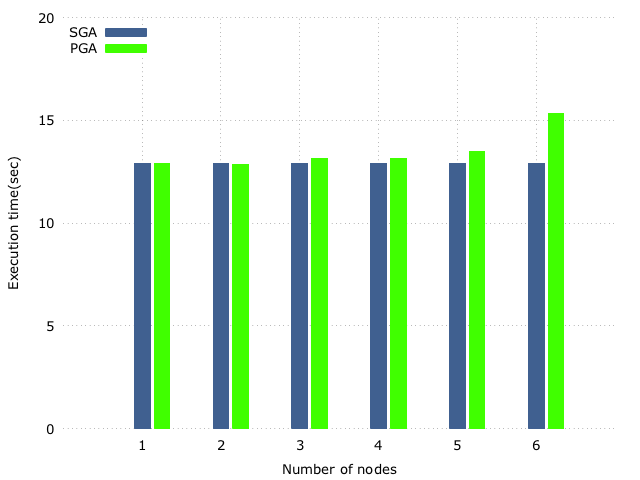
\includegraphics[width=.7 \linewidth]{stats_data_new/graphs/pga_xNodes_hist.png}
  \caption{Experiment 1 - Runtime comparison SGA vs PGA v1.}
  \end{center}\
\end{figure}

\begin{figure}[H]
\begin{center}
  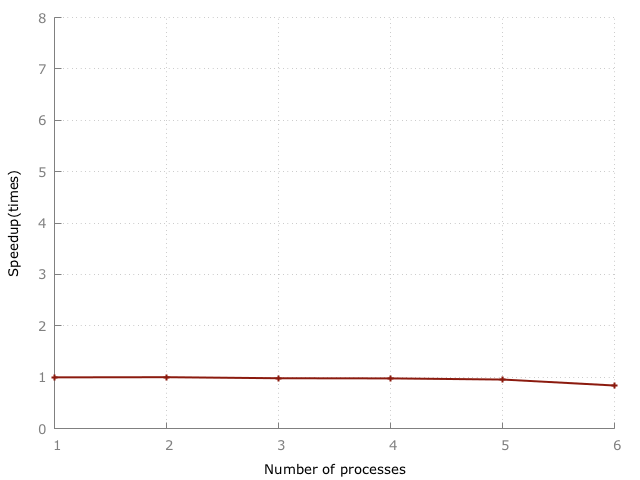
\includegraphics[width=.7 \linewidth]{stats_data_new/graphs/pga_xNodes_line.png}
  \caption{Experiment 1: Speedup graph SGA vs PGA v1.}
  \end{center}\
\end{figure}

\subsubsection{Discussion}
This experiment shows that there is no speedup gain when the number of processes were increased. That is because the communication overhead for MPI increases as the number of processes increases.

\subsection{Experiment 2: Varying population size}

\subsubsection{Objective}
Comparison of PGA v1 runtime vs. SGA runtime by varying the population size using 6 processes for PGA program.

\begin{table}[H]
\centering
\caption{Experiment 2 data using PGA v1}
\label{tab:pga1_pop}
\begin{tabular}{|l|l|l|l|}
\hline
\# population & SGA     & PGA     & speedup \\ \hline
1000          & 0.57    & 0.6827  & 0.835   \\ \hline
2000          & 2.1459  & 2.3018  & 0.9323  \\ \hline
3000          & 4.7258  & 4.9238  & 0.9598  \\ \hline
4000          & 8.2976  & 11.0389 & 0.7517  \\ \hline
5000          & 12.8896 & 15.7361 & 0.8191  \\ \hline
6000          & 18.4622 & 20.249  & 0.9118  \\ \hline
7000          & 25.0535 & 26.8225 & 0.934   \\ \hline
8000          & 32.667  & 36.5315 & 0.8942  \\ \hline
9000          & 41.3425 & 42.1336 & 0.9812  \\ \hline
10000         & 50.8885 & 51.9144 & 0.9802  \\ \hline
\end{tabular}
\end{table}

\begin{figure}[H]
\begin{center}
  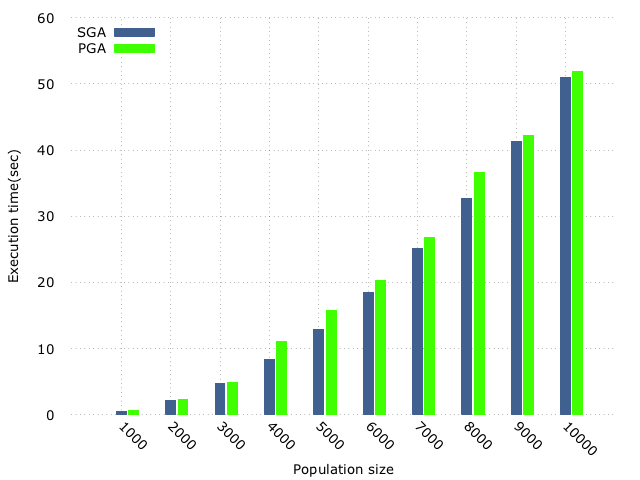
\includegraphics[width=.7 \linewidth]{stats_data_new/graphs/pga_xPop_hist.png}
  \caption{Experiment 2 - Runtime comparison SGA vs. PGA v1.}
  \end{center}\
\end{figure}

\begin{figure}[H]
\begin{center}
  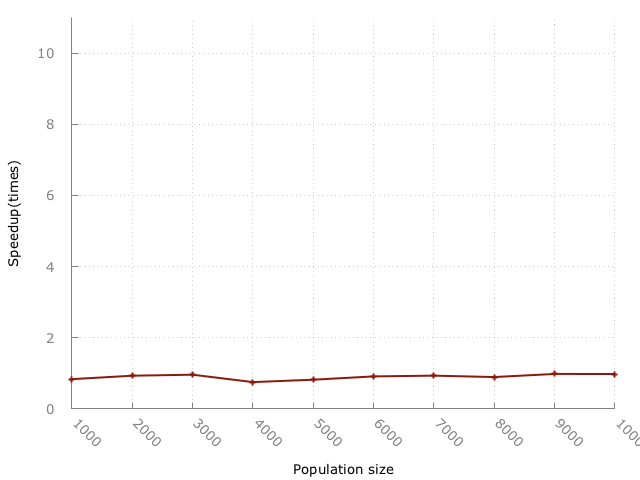
\includegraphics[width=.7 \linewidth]{stats_data_new/graphs/pga_xPop_line.png}
  \caption{Experiment 2 - Speedup graph SGA vs. PGA v1.}
  \end{center}\
\end{figure}

\subsubsection{Discussion}
This experiment shows that there is no speedup gain as the population size were increased either. Again, this shows that the communication overhead for MPI has significant impact of overall runtime of the program. This overhead increases with population size.

\section{Experiments using PGA v2}
%============PGA v2 ==============

\subsection{Experiment 3: Varying number of processes}

\subsubsection{Objective}
Comparison of PGA v2 runtime vs. SGA runtime by varying the number of processes the work is distributed for the PGA program to see the speedup gain using a fixed population size 5000.

\begin{table}[H]
\centering
\caption{Experiment 3 data using PGA v2}
\label{tab:pga2_node}
\begin{tabular}{|l|l|l|l|}
\hline
\# Process(es) & SGA     & PGA     & speedup \\ \hline
1        & 12.8795 & 12.8713 & 1.0006  \\ \hline
2        & 12.8795 & 8.6353  & 1.4915  \\ \hline
3        & 12.8795 & 6.5845  & 1.956   \\ \hline
4        & 12.8795 & 6.7115  & 1.919   \\ \hline
5        & 12.8795 & 5.1471  & 2.5023  \\ \hline
6        & 12.8795 & 5.0748  & 2.538   \\ \hline
\end{tabular}
\end{table}

\begin{figure}[H]
\begin{center}
  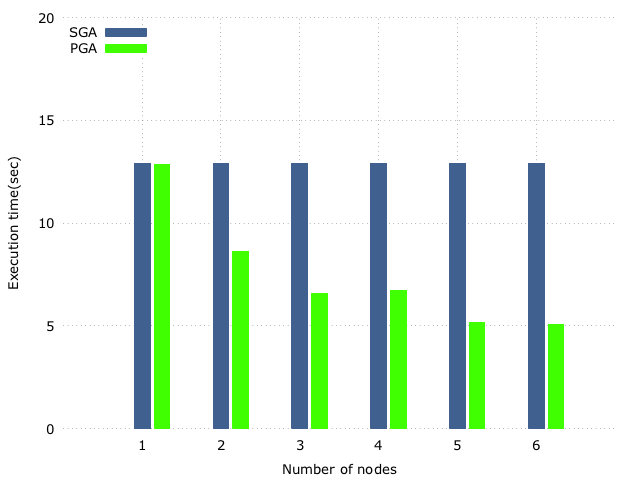
\includegraphics[width=.7 \linewidth]{stats_data_new/graphs/pga_global_xNodes_hist.png}
  \caption{Experiment 3 - Runtime comparison SGA vs. PGA v2.}
  \end{center}\
\end{figure}

\begin{figure}[H]
\begin{center}
  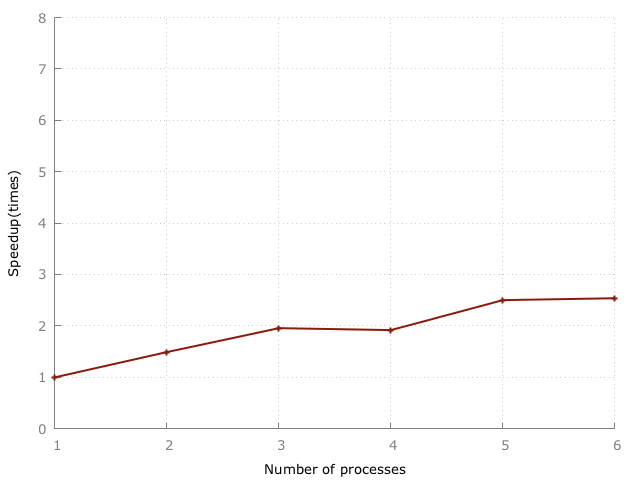
\includegraphics[width=.7 \linewidth]{stats_data_new/graphs/pga_global_xNodes_line.png}
  \caption{Experiment 3 - Speedup graph SGA vs. PGA v2.}
  \end{center}\
\end{figure}

\subsubsection{Discussion}
With this experiment we observed that there is speedup gain with PGA v2 as number of processes increases. However, this gain is much lower than expected with 6 processes given that the MPI collective communication routine were used for this implementation to reduce the communication overhead of PGA v1.

\subsection{Experiment 4: Varying population size}

\subsubsection{Objective}
Comparison of PGA v2 runtime vs. SGA runtime varying the number the population size using 6 processes for PGA program.

\begin{table}[H]
\centering
\caption{Experiment 4 data using PGA v2}
\label{tab:pga2_pop}
\begin{tabular}{|l|l|l|l|}
\hline
\# population & SGA     & PGA     & speedup \\ \hline
1000          & 0.5698  & 0.4957  & 1.1495  \\ \hline
2000          & 2.146   & 1.3006  & 1.65    \\ \hline
3000          & 4.7207  & 2.2022  & 2.1437  \\ \hline
4000          & 8.3287  & 3.4562  & 2.4098  \\ \hline
5000          & 12.8959 & 4.8998  & 2.6319  \\ \hline
6000          & 18.4703 & 7.016   & 2.6326  \\ \hline
7000          & 25.0758 & 21.6343 & 1.1591  \\ \hline
8000          & 32.7814 & 28.134  & 1.1652  \\ \hline
9000          & 41.2779 & 31.5602 & 1.3079  \\ \hline
10000         & 50.9403 & 44.5325 & 1.1439  \\ \hline
\end{tabular}
\end{table}

\begin{figure}[H]
\begin{center}
  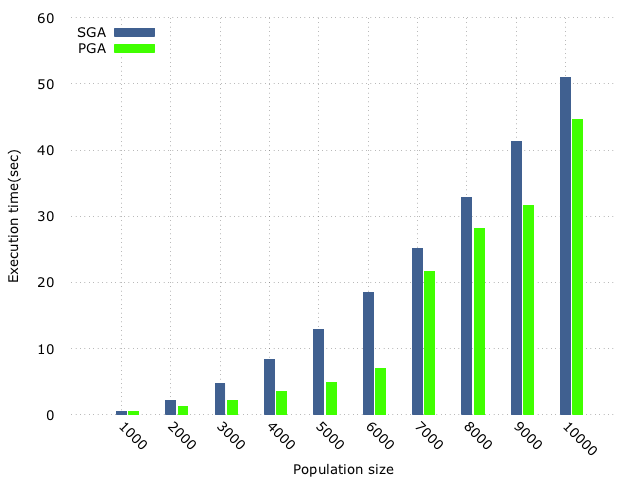
\includegraphics[width=.7 \linewidth]{stats_data_new/graphs/pga_global_xPop_hist.png}
  \caption{Experiment 4 - Runtime comparison SGA vs. PGA v2.}
  \end{center}\
\end{figure}

\begin{figure}[H]
\begin{center}
  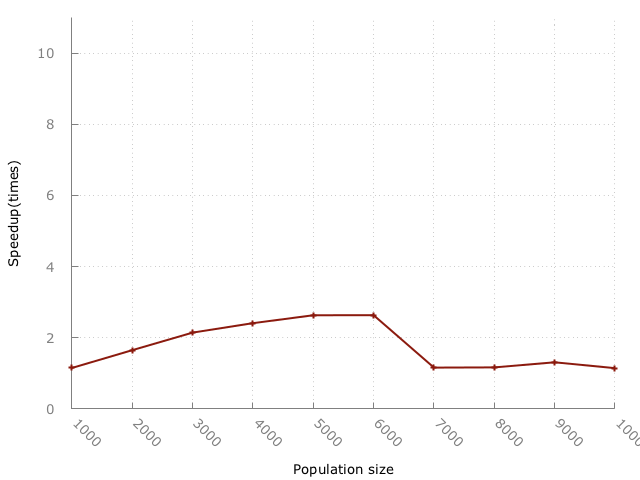
\includegraphics[width=.7 \linewidth]{stats_data_new/graphs/pga_global_xPop_line.png}
  \caption{Experiment 4 - Speedup graph SGA vs PGA v2.}
  \label{fig:exp2_pgav2_graph}
  \end{center}\
\end{figure}

\subsubsection{Discussion}
Result of this experiment is very interesting as we can see from the graph shown in Figure \ref{fig:exp2_pgav2_graph}. In Experiment 3 we saw somewhat of a steady gain in speedup for a fixed population size of 5000. But here we see as population size is increased (after 6000), there is a decrease in speedup. To find out the possible issue that may cause this behaviour, a running time analysis was carried to identify the problem that was discussed in section \ref{pga_runtime_analysis}. It was identified that the selection procedure had a running time complexity of $\mathcal{O}(n^2)$. As population size is increased after a certain threshold (6000 in this experiment) the runtime to this program started to increase rapidly which degraded the overall performance of speedup of this program by parallelising with many processes.

\section{Experiments using PGA v3}
%============PGA v3 ==============

\subsection{Experiment 5: Varying number of processes}

\subsubsection{Objective}
Comparison of PGA v3 runtime vs. SGA runtime varying the number of processes the work is distributed for the PGA program to see the speedup gain using a fixed population size 5000.

\begin{table}[H]
\centering
\caption{Experiment 5 data using PGA v3}
\label{tab:pga3_node}
\begin{tabular}{|l|l|l|l|}
\hline
\# Process(es) & SGA    & PGA     & speedup(SGA/PGA) \\ \hline
1        & 12.878 & 13.3253 & 0.9664           \\ \hline
2        & 12.878 & 3.5889  & 3.5883           \\ \hline
3        & 12.878 & 3.511   & 3.6679           \\ \hline
4        & 12.878 & 2.1288  & 6.0495           \\ \hline
5        & 12.878 & 1.9293  & 6.675            \\ \hline
6        & 12.878 & 1.7058  & 7.5496           \\ \hline
\end{tabular}
\end{table}


\begin{figure}[H]
\begin{center}
  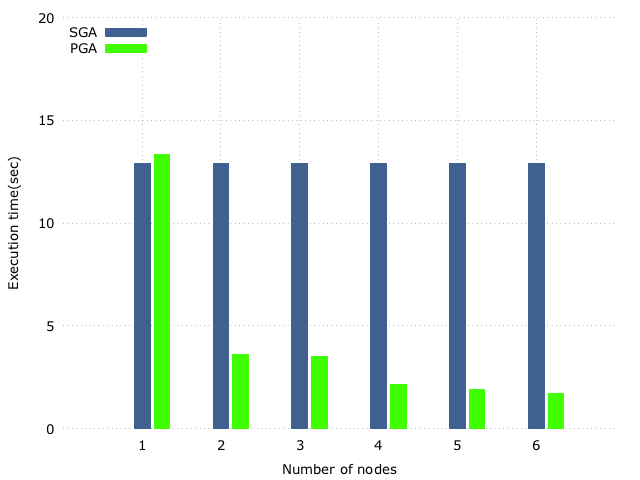
\includegraphics[width=.7 \linewidth]{stats_data_new/graphs/pga_partial_xNodes_hist.png}
  \caption{Experiment 5 - Runtime comparison SGA vs. PGA v3.}
  \end{center}\
\end{figure}

\begin{figure}[H]
\begin{center}
  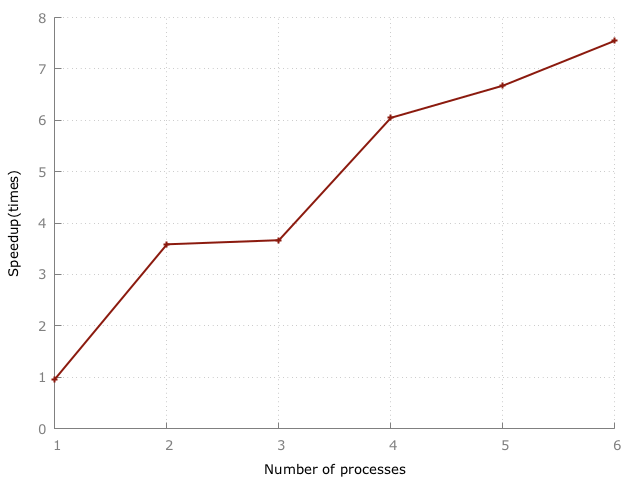
\includegraphics[width=.7 \linewidth]{stats_data_new/graphs/pga_partial_xNodes_line.png}
  \caption{Experiment 5 - Speedup graph SGA vs. PGA v3.}
  \end{center}\
\end{figure}

\subsubsection{Discussion}
In this experiment we see a better improvement in overall speedup. But the curb of the gain is not smooth. From 2 processes to 3 processes there is not much gain but from 3 processes to 4 processes we see a sudden spike. Only explanation of this could be the fact that how MPI Process Manager creates process in the cluster. With the hosts file configuration shown in Section \ref{lst:config_hydra}, Hydra (MPI Process Manager) runs 2 processes in one physical node. So, with both 3 and 4 processes we have 2 physical nodes running this program. Most likely, the underlying cache management and network overheard per node have something to do with the irregular performance variance. Running 2 processes in same physical node would have advantages of less network overheads and better caching over running a single process. This could only be confirmed by profiling this program using TAU(Tuning and Analysis Utilities) to further analyse it and find out any underlying cause should we had more time.


\subsection{Experiment 6: Varying population size}

\subsubsection{Objective}
Comparison of PGA v3 runtime vs. SGA runtime varying the number the population size using 6 processes for PGA program.

\begin{table}[H]
\centering
\caption{Experiment 6 data using PGA v2}
\label{tab:pga3_pop}
\begin{tabular}{|l|l|l|l|}
\hline
\# population & SGA     & PGA    & speedup \\ \hline
1000          & 0.5694  & 0.3594 & 1.5844  \\ \hline
2000          & 2.1434  & 0.6143 & 3.4894  \\ \hline
3000          & 4.7145  & 0.9252 & 5.0954  \\ \hline
4000          & 8.3063  & 1.3231 & 6.2777  \\ \hline
5000          & 12.9011 & 1.6985 & 7.5957  \\ \hline
6000          & 18.5207 & 2.2113 & 8.3753  \\ \hline
7000          & 25.1309 & 2.7727 & 9.0636  \\ \hline
8000          & 32.6705 & 3.4446 & 9.4846  \\ \hline
9000          & 41.2867 & 4.2053 & 9.8179  \\ \hline
10000         & 50.9591 & 5.0311 & 10.1288 \\ \hline
\end{tabular}
\end{table}

\begin{figure}[H]
\begin{center}
  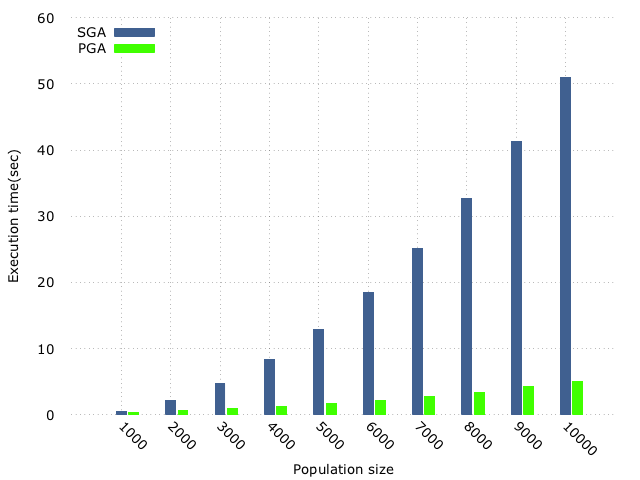
\includegraphics[width=.7 \linewidth]{stats_data_new/graphs/pga_partial_xPop_hist.png}
  \caption{Experiment 6 - Runtime comparison SGA vs. PGA v3.}
  \end{center}\
\end{figure}

\begin{figure}[H]
\begin{center}
  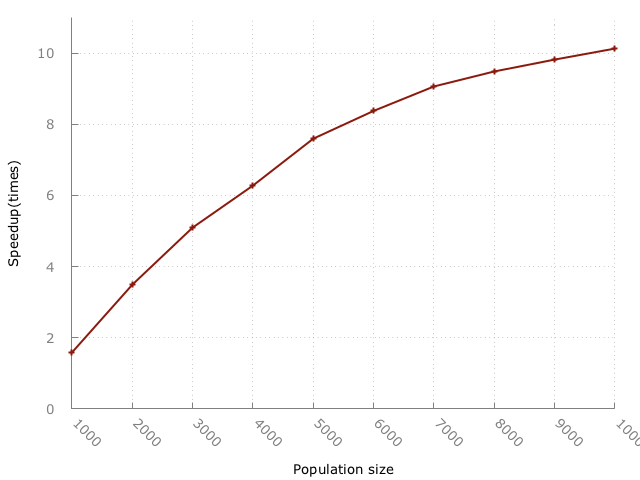
\includegraphics[width=.7 \linewidth]{stats_data_new/graphs/pga_partial_xPop_line.png}
  \caption{Experiment 6 - Speedup graph SGA vs. PGA v3.}
  \end{center}\
\end{figure}

\subsubsection{Discussion}
With this experiment we can see there is a consistent speedup gain with PGA v3 compared to the SGA program as population size is increased. Even though the outcome of this experiment is as expected, the results are taken as speculative until further experiments are done using different parameters. Profiling of this program also needs to be done to see a consistent and reliable outcome.
